\section{High Granularity Calorimeter} \label{section:simulations_hgc}
The High Granularity Calorimeter, \cite{Magnan:2017exp}, (HGC) model that is built and analyzed in this chapter, although implements the proper geometry, borrows all the basics from the CALICE Silicon-Tungsten, \cite{Adloff:2008aa}, (SiW) system. Moreover, both {\sc HGC} and {\sc CALICE} SiW terms are used interchangeably, because, although {\sc HGC} has both electromagnetic and hadronic parts, for the sake of discussion, the hadronic part is omitted. Figure \ref{fig:simulations_hgcexamples} shows a custom {\sc Geant4} built full CMS scale High Granularity Calorimeter as CMS Endcap system. The HGC has been one of the potential candidates for the CMS Phase 2 upgrade.
\begin{figure}[htbp]
    \centering
    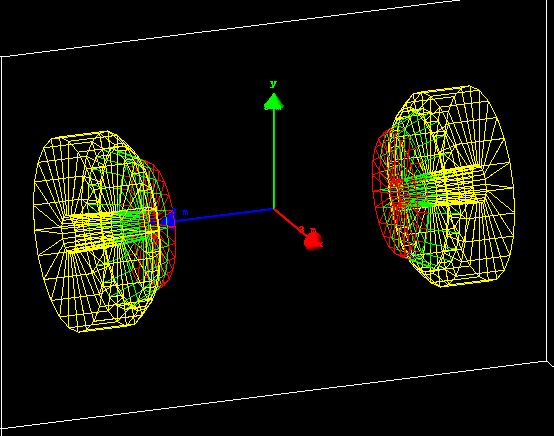
\includegraphics[width=0.9\textwidth]{figures/ch_simulations/hgc/detetor_3d/HGC_70_20.png}
    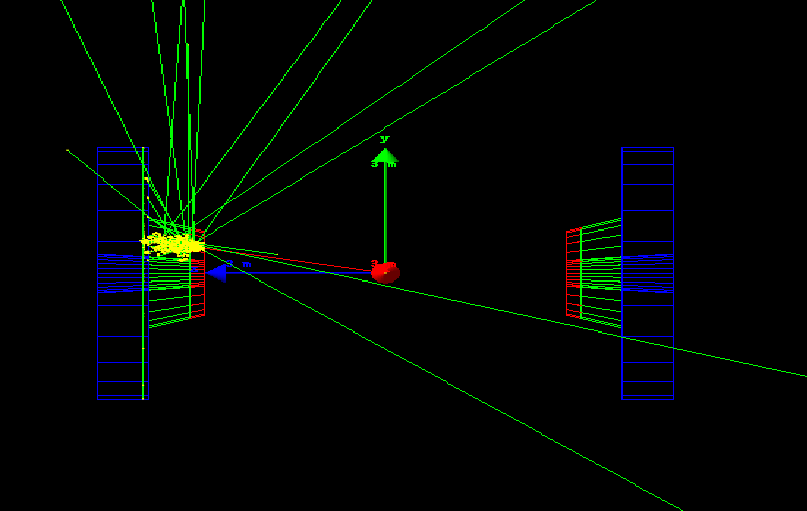
\includegraphics[width=0.9\textwidth]{figures/ch_simulations/hgc/detetor_3d/HGCal_1Event_NoSides.png}
    \caption{Full CMS Scale High Granularity Calorimeter (Top). Example of a Particle Gun response (Bottom)}
    \label{fig:simulations_hgcexamples}
 \end{figure}

\subsection{Physical Layout}
HGC consists of three parts: \textbf{Electromagnetic} (EM) calorimeter, \textbf{Front Hadron} (FH) and \textbf{Backing Hadron} (BH) Calorimeters. Both EM and FH have similar design principles: alternating layers of absorber and active materials mixed in together with a layer of electronics readout. Full geometry specification for the EM part can be summarized as follows:
\begin{itemize}
    \item 25 Radiation Length ($X_{0}$) Device
    \item In total 30 layers, where each layer is (absorber (W), active (Si), readout (G10/PCB)).
    \item First 10 layers have $0.5$ $X_{0}$ per layer
    \item Second 10 layers have $0.8$ $X_{0}$ per layer
    \item Third 10 layers have $1.2$ $X_{0}$ per layer
    \item XY-plane is subdivided into pads, with an area of each channel of 0.9 $cm^2$ for the first 20 layers and 1.8 $cm^2$ for the last 10.
\end{itemize}
Full specification for the FH part can be summarized as follows:
\begin{itemize}
    \item 4 Interaction length ($\lambda$) Device
    \item 12 layers of (absorber (W/Brass), active (Si), readout (G10/PCB)), each layer is $0.33$ $\lambda$
    \item XY-plane is also subdivided into small pads, with each covering an area of 1.8 $cm^2$
\end{itemize}

\subsection{Detector Readout} \label{subsection:simulations_hgc_readout}
The operating principle of SiW calorimeter is based on electron-hole pairs generated by a charged track traversing within the active material. For the purpose of simulation, assume a constant number of such holes per \SI{1}{\micro\metre} step (80 holes per \SI{1}{\micro\metre}), which is a valid assumption that has been previously used by {\sc CALICE} SiW Electromagnetic Calorimeter \cite{Adloff:2008aa}. Equation~\ref{eq:simulation_hgc_responsePerCell} summarizes the computation of the response for a single pad per event.
\begin{center}
    \begin{equation}
        \label{eq:simulation_hgc_responsePerCell}
        {R(cell)} = {\sum_{n=1}^{steps} \frac{80\times \Delta x}{1\mu m}}
 %       \caption{Response per cell. $\Delta$x is a single step size}
   \end{equation}
\end{center}

\subsection{Simulation}
The goal of the modeling is to establish the performance characteristics of the calorimeter system: response linearity and energy resolution. For that electron Particle Gun with varying energies is used. Each event corresponds to shooting a single $e^-$ of certain energy, performing all the tracking for all of the shower particles and recording all of the results as discussed in Section~\ref{subsection:simulations_hgc_readout}. It is important to point out that each primary particle enters the detector at an angle of normal incidence for the purpose of precise control of the simulation environment. Figure~\ref{fig:simulations_hgc_scatter60} provides an example of a shower distribution for a single event.
\begin{figure}[htbp]
    \centering
    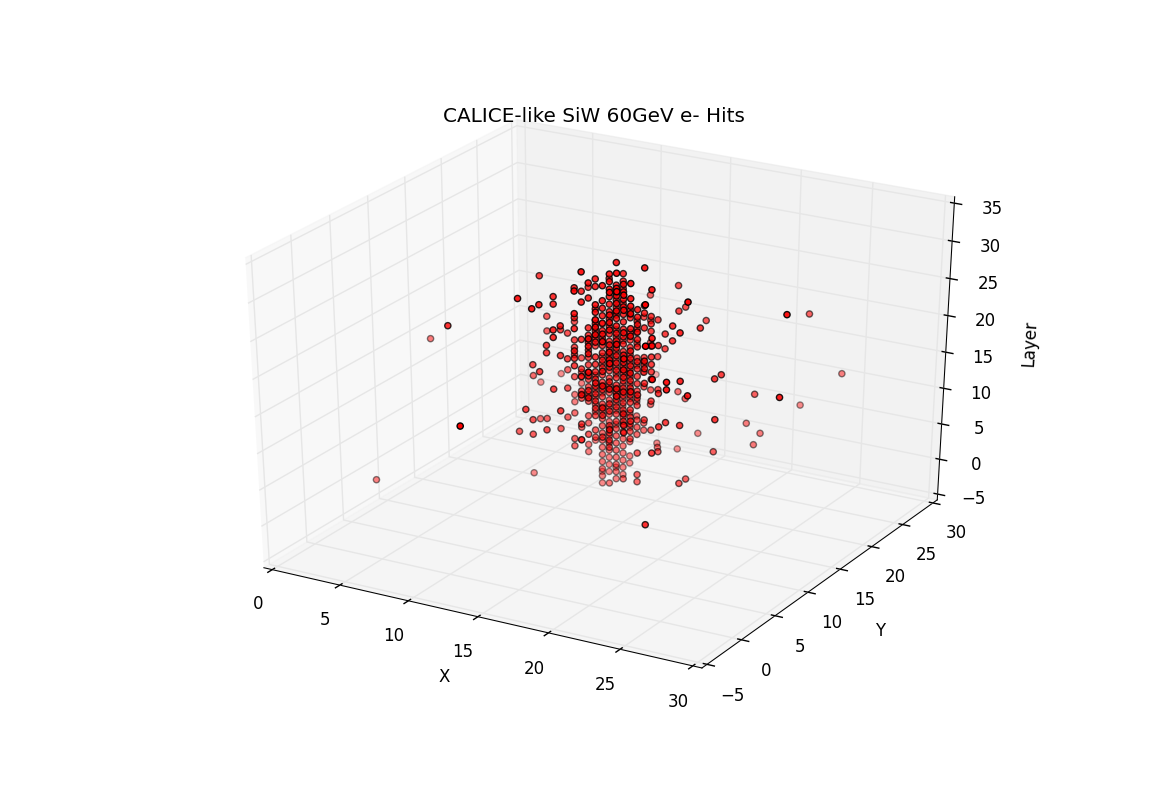
\includegraphics[width=0.9\textwidth]{figures/ch_simulations/hgc/scatter_3d/scatter_3D_60GeV.png}
    \caption{An example of a shower distribution within {\sc HGC} for an incident 60 GeV $e^-$}
    \label{fig:simulations_hgc_scatter60}
 \end{figure}

\subsection{Analysis}
The objective of the readout analysis is to establish calorimeter performance characteristics: linearity of response and energy resolution. Not all systems are linear and intrinsically SiW calorimeters are not linear in response. The reason for desirability of this characteristic is the ability to easily calibrate the device. In other words, given a linear system, the conversion of the raw response to energy is trivially established. In summary, the following steps are to be followed to establish the performance characteristics:
\begin{itemize}
    \item Compute Total Response. Use Equation \ref{eq:simulations_hgc_responsePerCell}
    \item Compute the Energy due to the calorimeter response. Use Equation \ref{eq:simulations_hgc_totalResponse}.
    \item Overlay particle gun energy with total response as in Figure \ref{fig:simulations_hgc_pblinearityresolution}. Perform a linear fit and extract the calibration coefficient.
    \item Using the derived calibration coefficient, for each generated event, compute the Energy due to the response. Figure \ref{fig:simulations_hgc_pbenergyreco} shows the reconstructed energy distributions.
    \item Using Equation~\ref{eq:simulations_hgc_resolution}, compute and overlay Resolution with the incident energy. Perform the fit using Equation~\ref{eq:simulations_hgc_resolutionfitfunc}.
\end{itemize}
\begin{subequations}\label{eq:simulations_hgc_definitions}
\begin{align}
    E& = {CC} \times {Raw Response}. = {CC} \times {\sum_{i=1}^{n_{layers}} w_i \times  R_{i}}\label{eq:simulations_hgc_totalResponse}\\
    {Resolution}& = {\frac{\sigma_E}{\mu_E}}\label{eq:simulations_hgc_resolution}\\
    {f(x)}& = {\sqrt{\frac{\alpha^2}{x} + C^2}}\label{eq:simulations_hgc_resolutionfitfunc}
\end{align}
\end{subequations}
where in Equation \ref{eq:simulations_hgc_resolutionfitfunc}, $\alpha$ is the term that represents the level of intrinsic statistical fluctuations of the calorimeter and $C$, constant or asymptotic term, sets the limits of the calorimeter at higher energies.

\subsection{Results}
Following the procedure described just above, first obtain the results for the linearity of {\sc HGC} in Figure \ref{fig:simulations_hgc_pblinearity}. The yield per $1$ GeV, about $4.4$ $\times$ $10^6$, is the extracted Calibration Coefficient (CC). As it can be observed - the electromagnetic response is highly linear!
 \begin{figure}[htbp]
    \centering
    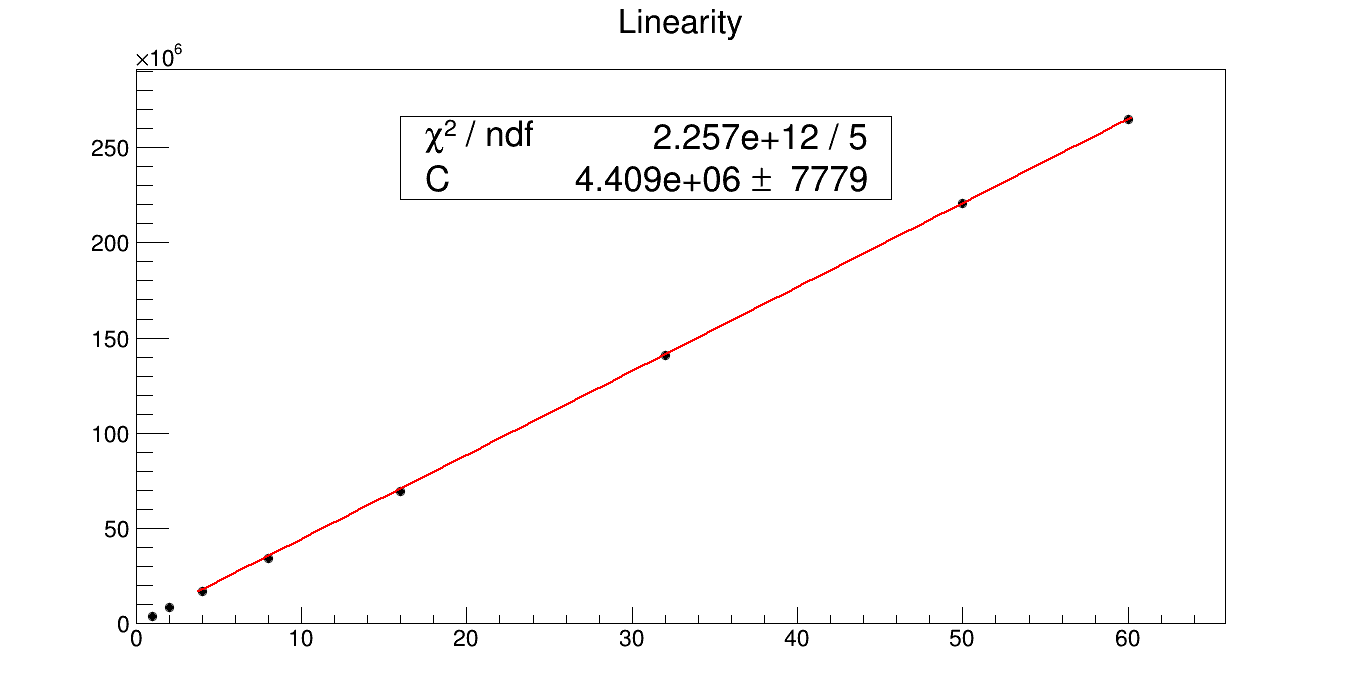
\includegraphics[width=0.95\textwidth]{figures/ch_simulations/hgc/performance/Pb/Linearity.png}
    \caption{The linearity graph of the Electromagnetic component of the {\sc HGC}. Shows the dependence of the total calorimeter response as a function of the energy of the incident e$^-$}
    \label{fig:simulations_hgc_pblinearity}
 \end{figure}

Furthermore, applying the obtained the Calibration Coefficient for the purpose of the energy reconstruction according to the Equation~\ref{eq:simulations_hgc_definitions} results in the energy distributions shown in Figure \ref{fig:simulations_hgc_pbenergyreco}. Electron particle gun with eight different energies have been used. A Gaussian fit is performed in order to extract the mean and the width of the reconstructed energy distributions.
\begin{figure}[htbp]
    \centering
    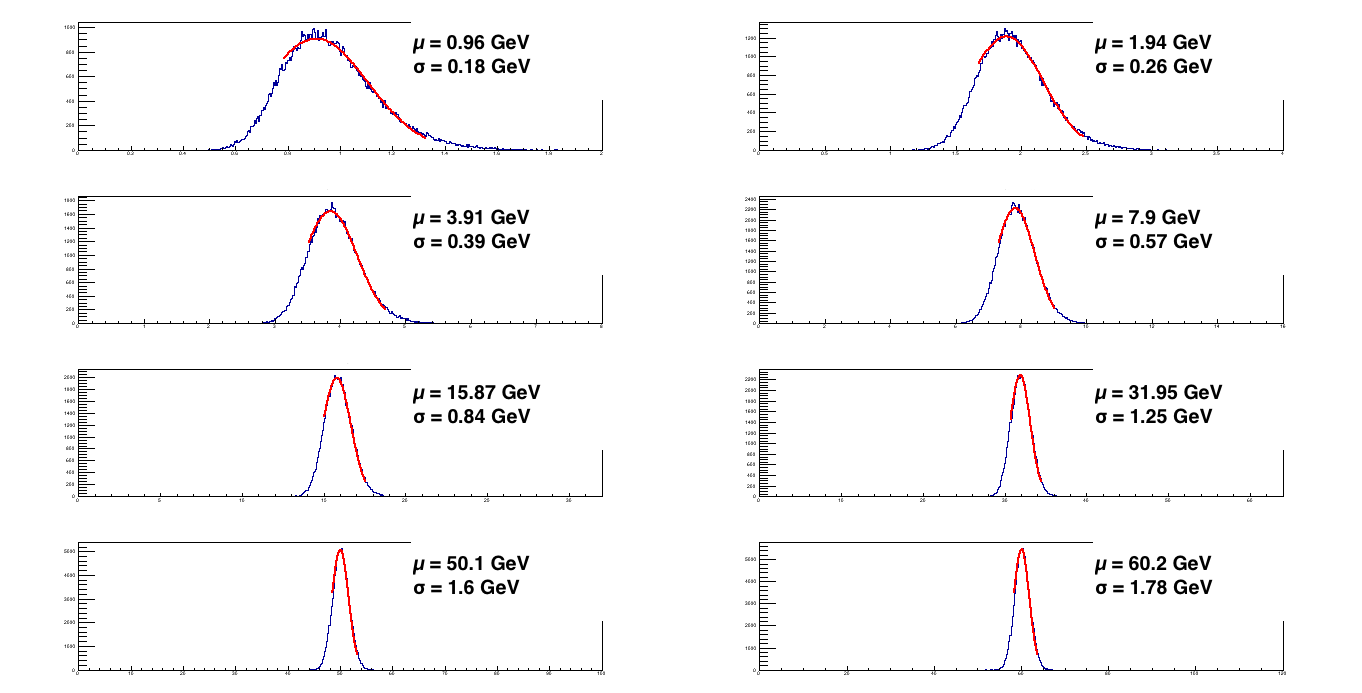
\includegraphics[width=0.95\textwidth]{figures/ch_simulations/hgc/performance/Pb/EnergyRECO.png}
    \caption{The {\sc HGC} Reconstructed Energy Distributions. Electron particle gun used with eight different energies: 1 GeV, 2 GeV, 4 GeV, 8 GeV, 16 GeV, 32 GeV, 50 GeV, 60 GeV}
    \label{fig:simulations_hgc_pbenergyreco}
 \end{figure}

And, finally, the energy resolution results are shown in Figure \ref{fig:simulations_hgc_pbresolution}. The asymptotic energy resolution of the HGC electromagnetic component is at 1\%.
 \begin{figure}[htbp]
    \centering
    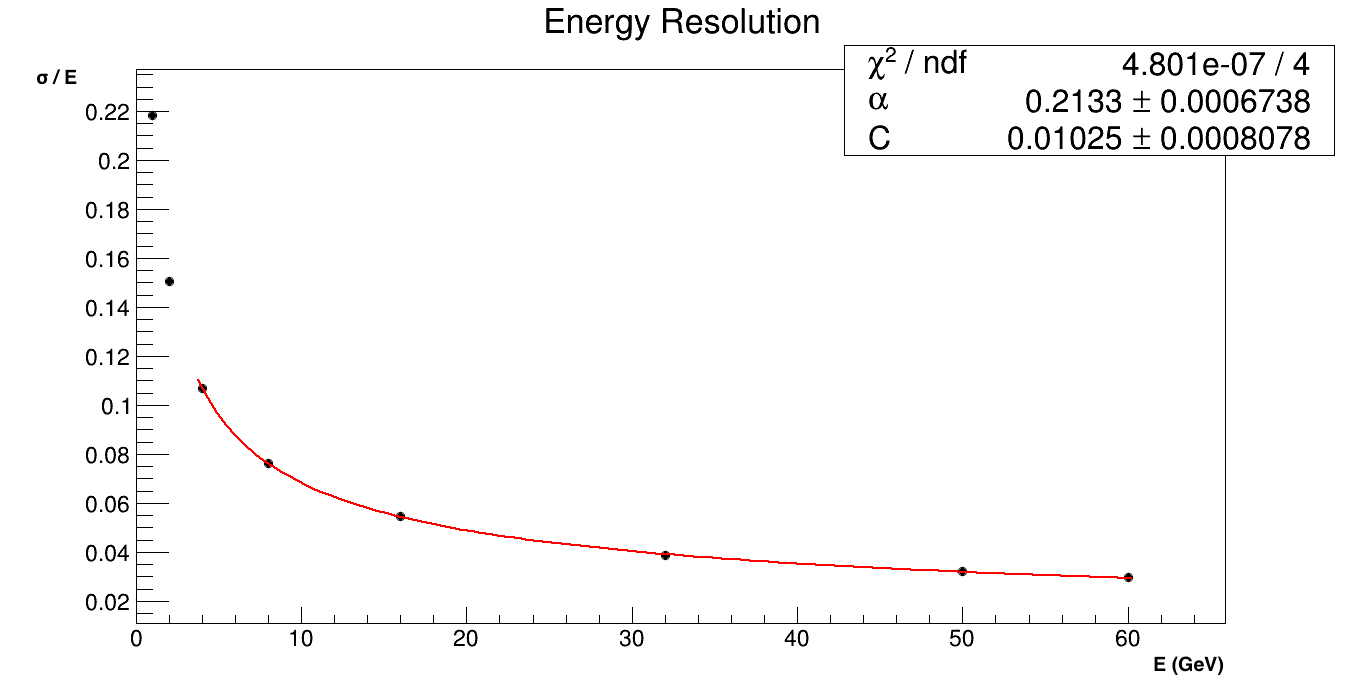
\includegraphics[width=0.95\textwidth]{figures/ch_simulations/hgc/performance/Pb/Resolution.png}
    \caption{The {\sc HGC} Energy Resolution curve. Stochastic component $\alpha$ (0.21) determines the level of statistical fluctuations and C (1\%) shows the behavior of the system at high energies}
    \label{fig:simulations_hgc_pbresolution}
 \end{figure}